\section{The least loss with zeros}\label{sec:allzeros}

This section solves \cref{prob:zeros}. The answer is stronger than the
problem asks. For every phase $\theta\notin\pi\Z$ there is one passive system
whose attenuation is the least possible at every frequency of the band
simultaneously, among all passive systems with that argument, with or
without zeros. It has exactly one zero, on the imaginary axis, and it is
lossless off the band. For $\theta=\pi/2$ it is algebraic, and every quantity
is elementary.

\subsection{Statement}

We call a passive system $H$ \emph{admissible for} $\theta$ if it is regular
on the band in the sense of \cref{def:band} (the definition makes sense for
any passive system) and $\arg H\equiv\theta\pmod{2\pi}$ on $[a,b]$. The
admissible systems are exactly those of \cref{prob:zeros}. Since $-H$ is
passive whenever $H$ is, and $\arg(-H)=\arg H+\pi$, it suffices to treat
$0<\theta<\pi$. We use $r$, $h_g$, $v_g$, $\beta_g$, $B_\eta$ and $\delta$ as in
\cref{sec:extremal,sec:zeros}.

\begin{theorem}\label{thm:allzeros}
Let $0<\theta<\pi$. The equation
\begin{equation}\label{eq:etastar}
\int_a^b\frac{2\arctan(t/\eta)}{r(t)}\dd t=\theta\int_a^b\frac{\dd t}{r(t)}
\end{equation}
has exactly one root $\eta_\star\in(0,\eta_\theta)$. Put
\begin{gather*}
g_\sharp(\omega)=\theta-2\arctan\frac\omega{\eta_\star},\qquad
\Hs_\theta=-B_{\eta_\star}e^{ih_{g_\sharp}},\\
\as_\theta=v_{g_\sharp}\quad\text{on }[a,b].
\end{gather*}
\begin{enumerate}
\item[(i)] $\Hs_\theta$ is admissible for $\theta$. It has exactly one zero in
$\Cp$, at $i\eta_\star$, it is lossless on $\R\setminus S$, it satisfies
$\Hs_\theta(0)=1$ and $\Hs_\theta(iy)\to-1$ as $y\to\infty$, and its
attenuation $\as_\theta$ is positive on $(a,b)$ and vanishes at $a$ and $b$.
\item[(ii)] Every system $H$ admissible for $\theta$ satisfies
\begin{equation}\label{eq:pointwise}
\alpha(\omega)\ge\as_\theta(\omega)\qquad(a\le\omega\le b).
\end{equation}
If equality holds on a set of positive measure, then $H=\Hs_\theta$.
\item[(iii)] Consequently
\begin{equation}\label{eq:lambdaall}
\Lambda_{\mathrm{all}}(\theta)=\frac1{b-a}\int_a^b\as_\theta\dd\omega
=\theta\Lambda-\delta(\eta_\star)>0,
\end{equation}
the infimum is attained only by $\Hs_\theta$, and it is strictly smaller than
the mean attenuation of every system of \cref{prop:onezero}. For
$\pi<\theta<2\pi$, $\Lambda_{\mathrm{all}}(\theta)=\Lambda_{\mathrm{all}}(\theta-\pi)$,
attained only by $-\Hs_{\theta-\pi}$.
\end{enumerate}
\end{theorem}

The inequality \eqref{eq:pointwise} is pointwise. A single system is
optimal for the mean, for every weighted mean, for the worst frequency and
for the geometric mean at the same time (\cref{cor:allweights}). The
zero-free theory has the same feature for an affine phase
(\cref{thm:affine}), although its sum rule bounds only the mean; there the
constraint $\beta\ge0$ ties the frequencies of the band together, and
zeros remove it (\cref{rem:whypointwise}).

For a right angle everything is explicit.

\begin{theorem}\label{thm:rightangle}
Let $\theta=\pi/2$. Then $\eta_\star=\sqrt{ab}$, and
\begin{equation}\label{eq:Hright}
\Hs_{\pi/2}(z)=-\frac{z^2+ab}{R(z)+i(a+b)z},
\end{equation}
with $R$ as in \cref{lem:R}. Its attenuation is
\begin{equation}\label{eq:alpharight}
\begin{aligned}
\as_{\pi/2}(\omega)&=\log\frac{(a+b)\,\omega+r(\omega)}{\omega^2+ab}\\
&=2\operatorname{artanh}\sqrt{\frac{(\omega-a)(b-\omega)}{(\omega+a)(\omega+b)}} ,
\end{aligned}
\end{equation}
and
\begin{equation}\label{eq:lambdaright}
\int_a^b\as_{\pi/2}\dd\omega=\frac\pi2\big(\sqrt b-\sqrt a\big)^2,\quad
\Lambda_{\mathrm{all}}\Big(\frac\pi2\Big)=\frac\pi2\,\frac{\sqrt b-\sqrt a}{\sqrt b+\sqrt a}.
\end{equation}
The profile $\as_{\pi/2}$ is invariant under $\omega\mapsto ab/\omega$ and has
its only maximum at the geometric centre $\omega_0=\sqrt{ab}$, where
$\as_{\pi/2}(\omega_0)=\frac12\log(b/a)$. Hence every passive system with
$\arg H\equiv\pi/2\pmod\pi$ on $[a,b]$ that is regular on the band satisfies
\begin{equation}\label{eq:threedb}
\abs{H(\omega)}\le\frac{\omega^2+ab}{(a+b)\,\omega+r(\omega)},\qquad
\abs{H(\sqrt{ab})}^2\le\frac ab .
\end{equation}
\end{theorem}

For an octave, a passive system whose phase is a right angle at every
frequency of the band transmits at most half of the power at the geometric
centre: its loss there is at least $3.01$\,dB, and for a decade at least
$10$\,dB.\footnote{The power transmission is $\abs H^2\le a/b$, so the loss
is at least $10\log_{10}(b/a)$\,dB: $10\log_{10}2=3.0103$ and
$10\log_{10}10=10$.} The sum rule of the zero-free theory gives no bound of
this pointwise kind. The mean attenuation of
$\Hs_{\pi/2}$ over an octave is $\frac\pi2(3-2\sqrt2)=0.26951$\,Np, which is
$62.7\%$ of the zero-free value $\frac\pi2\Lambda=0.42966$. For a narrow band
the ratio of the two minimal means tends to $\sin\theta/\theta$
(\cref{cor:narrowzeros}), which is $2/\pi$ at a right angle.

\begin{table}[t]
\caption{The least mean attenuation over the octave $[1,2]$ of passive
systems with argument $\theta$ modulo $2\pi$, with or without zeros
(\cref{thm:allzeros}), the position of the zero of the optimal system
relative to $\eta_\theta=b\cot(\theta/2)$ of \cref{prop:onezero}, the ratio to
the zero-free value $\theta\Lambda$, and the least possible worst-frequency
attenuation $\max\as_\theta$.}
\label{tab:allzeros}
\centering
\small
\begin{tabular}{@{}rrrrr@{}}
\toprule
$\theta$ & $\eta_\star/\eta_\theta$ & $\Lambda_{\mathrm{all}}(\theta)$ &
$\Lambda_{\mathrm{all}}/\theta\Lambda$ & $\max\as_\theta$ \\
\midrule
$0.5$    & $0.72576$ & $0.13090$ & $0.9571$ & $0.16677$ \\
$1$      & $0.71853$ & $0.22860$ & $0.8357$ & $0.29204$ \\
$\pi/2$  & $0.70711$ & $0.26951$ & $0.6272$ & $0.34657$ \\
$2$      & $0.69843$ & $0.24357$ & $0.4452$ & $0.31540$ \\
$2.5$    & $0.69050$ & $0.15941$ & $0.2331$ & $0.20805$ \\
\bottomrule
\end{tabular}
\end{table}

\Cref{tab:allzeros} gives the octave values, and \cref{fig:allzeros} the
optimal profiles. Comparing with \cref{tab:zeros}: the optimal system beats
the one-zero system $H_{\eta_\theta}$ for every $\theta$, by $2.6\%$ at
$\theta=0.5$ and $22\%$ at $\theta=\pi/2$, and for $\theta\ge2$ it also beats
the lead branch. Its zero sits closer to the origin than $\eta_\theta$, so that
the phase $g_\sharp$ of its zero-free factor is negative on part of the band,
which \cref{lem:positivity} does not allow. At $\theta=\pi/2$ the ratio
$\eta_\star/\eta_\theta$ is $\sqrt{a/b}$, by \cref{thm:rightangle}.

\begin{figure}[t]
\centering
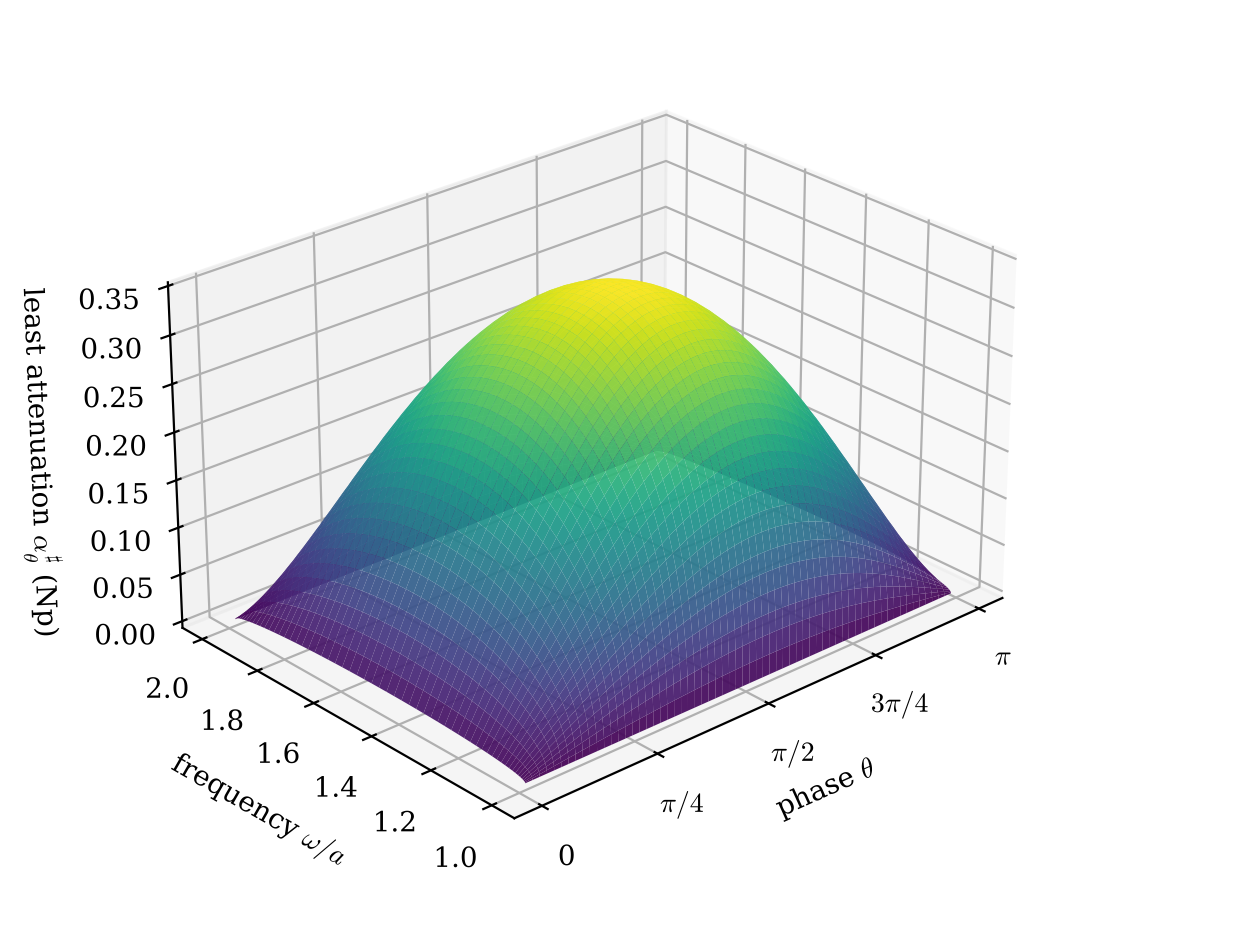
\includegraphics[width=\columnwidth]{figures/fig_allzeros.png}
\caption{The least attenuation $\as_\theta(\omega)$ at each frequency of the
octave, over the phase $\theta\in(0,\pi)$ (\cref{thm:allzeros}). No passive
system with argument $\theta$ on the band lies below the surface at any
frequency. The black curve is the closed form \eqref{eq:alpharight} at
$\theta=\pi/2$, with its peak $\frac12\log2$ at $\omega=\sqrt2$.}
\label{fig:allzeros}
\end{figure}

\begin{figure}[t]
\centering
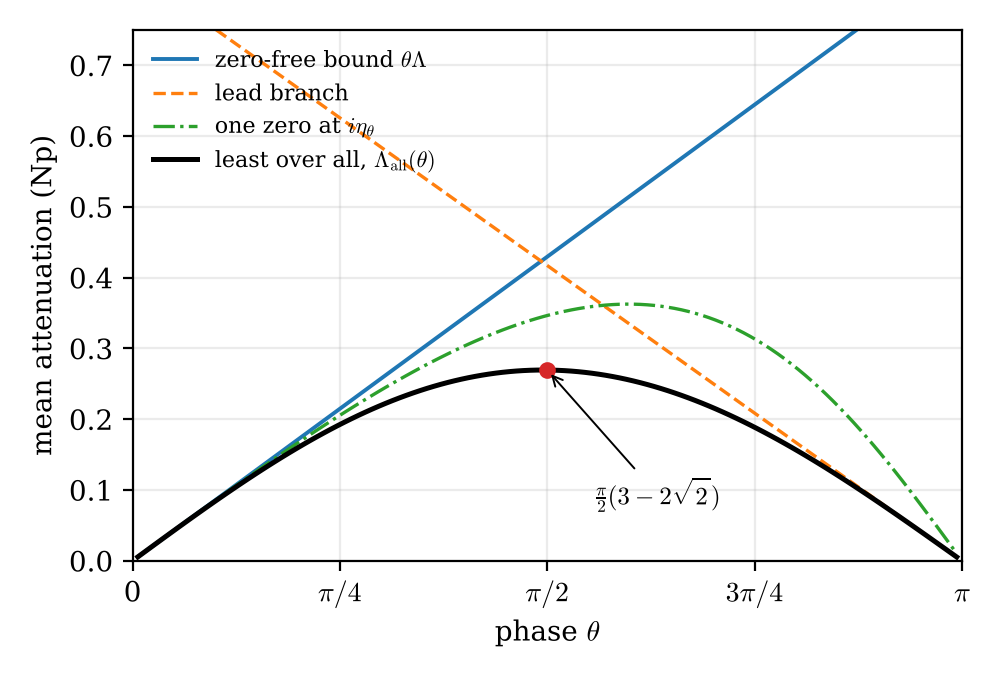
\includegraphics[width=\columnwidth]{figures/fig_lambdaall.png}
\caption{Mean attenuation over the octave against the phase $\theta$: the
zero-free bound $\theta\Lambda$ (\cref{thm:main}), the lead branch of
\cref{tab:zeros}, the one-zero system $H_{\eta_\theta}$
(\cref{prop:onezero}), and the exact minimum $\Lambda_{\mathrm{all}}(\theta)$
over all passive systems (\cref{thm:allzeros}). The dot marks the closed form
$\frac\pi2(3-2\sqrt2)$ at $\theta=\pi/2$.}
\label{fig:lambdaall}
\end{figure}

\subsection{A change of variables}

The phase condition $\arg H\equiv\theta$ is not linear in $\log H$ once
zeros are allowed, since $\log H$ is then not defined. A M\"obius
transformation of the values removes this difficulty.

\begin{lemma}\label{lem:transform}
Let $0<\theta<\pi$, let $H$ be a passive system that is not constant, and
put
\begin{equation}\label{eq:F}
F=e^{-i\theta}\,\frac{H-e^{i\theta}}{H-e^{-i\theta}},\qquad
H=\frac{F-e^{i\theta}}{e^{i\theta}F-1}.
\end{equation}
\begin{enumerate}
\item[(i)] $F$ is analytic in $\Cp$ with values in $\Cp$, and
$F(-\bar z)=1/\overline{F(z)}$. The function $\zeta=\log F$, with
$0<\Im\zeta<\pi$, satisfies $\zeta(-\bar z)=-\overline{\zeta(z)}$, and
\begin{equation}\label{eq:zetarep}
\zeta(z)=\frac1\pi\int_0^\infty g(t)\,\frac{2z}{t^2-z^2}\dd t ,
\end{equation}
where $g(t)=\Im\zeta(t+i0)\in[0,\pi]$ for almost every $t>0$. In
particular $\Re\zeta=0$ on $i\R_+$.
\item[(ii)] Conversely, if $F$ is analytic in $\Cp$ with values in $\Cp$ and
$F(-\bar z)=1/\overline{F(z)}$, then \eqref{eq:F} defines a passive system.
\item[(iii)] $\abs H=1$ at a point $t\in\R$ where $H$ is continuous if and
only if $F(t)$ is real there, and then $g(t)\in\{0,\pi\}$. The zeros of $H$
are the points where $F=e^{i\theta}$.
\item[(iv)] Let $H(\omega)=e^{i\theta-\alpha}$ with $\alpha>0$ at a point
$\omega$ of the band, and write $\zeta=u+iv$ there. (If $\alpha=0$, then $F=0$.)
Then
\begin{equation}\label{eq:bandcurve}
\frac1F=\cos\theta-i\sin\theta\coth\frac\alpha2,\qquad
e^u\cos\theta=\cos v,
\end{equation}
$u<0$, $v$ lies strictly between $\theta$ and $\pi/2$ (or $v=\pi/2$ if
$\theta=\pi/2$), and
\begin{equation}\label{eq:Au}
\alpha=A_\theta(u),\qquad
A_\theta(u)=2\operatorname{artanh}\frac{e^u\sin\theta}{\sqrt{1-e^{2u}\cos^2\theta}},
\end{equation}
where $A_\theta$ is a strictly increasing bijection of $(-\infty,0)$ onto
$(0,\infty)$. Conversely, a value $1/F$ of the form \eqref{eq:bandcurve}
with $\alpha>0$ corresponds to $H=e^{i\theta-\alpha}$.
\end{enumerate}
\end{lemma}

\begin{proof}
(i) Since $H$ is not constant, $\abs H<1$ in $\Cp$ by the maximum principle,
so $H\ne e^{\pm i\theta}$ there. The M\"obius map
$w\mapsto e^{-i\theta}(w-e^{i\theta})/(w-e^{-i\theta})$ sends the unit circle into
the real line\footnote{For $w=e^{i\phi}$,
$e^{i\phi}-e^{i\theta}=2ie^{i(\phi+\theta)/2}\sin\frac{\phi-\theta}2$ and
$e^{i\phi}-e^{-i\theta}=2ie^{i(\phi-\theta)/2}\sin\frac{\phi+\theta}2$, so the
image is $\sin\frac{\phi-\theta}2/\sin\frac{\phi+\theta}2\in\R$.} and $0$ to
$e^{i\theta}\in\Cp$, so it maps the open disc onto $\Cp$. The symmetry
$H(-\bar z)=\overline{H(z)}$ gives
$F(-\bar z)=e^{-i\theta}(\bar H-e^{i\theta})/(\bar H-e^{-i\theta})
=1/\overline{F(z)}$, hence the symmetry of $\zeta$. The function $\zeta$ is a
Herglotz function with bounded imaginary part, so in \eqref{eq:herglotz}
$\beta=0$ and $\dd\mu=\pi^{-1}g\dd t$ with $g$ the boundary values of $\Im\zeta$
\cite[Ch.~I]{garnett}. On $i\R_+$ the symmetry reads $\zeta=-\bar\zeta$, so
$\Re\zeta=0$ there and $c=\Re\zeta(i)=0$. The symmetry also makes $g$ even,
and folding the integral over $\R$ onto $(0,\infty)$ with
$\frac1{t-z}-\frac1{-t-z}=\frac{2z}{t^2-z^2}$ gives \eqref{eq:zetarep}; the
terms $t/(1+t^2)$ cancel.
(ii) The inverse M\"obius map in \eqref{eq:F} sends $\Cp$ into the open unit
disc, and the symmetry of $H$ follows by reversing the computation in (i).
(iii) The M\"obius map sends the unit circle onto the real line, and
$H=0$ exactly when $F=e^{-i\theta}(-e^{i\theta})/(-e^{-i\theta})=e^{i\theta}$.
(iv) Substituting $H=e^{i\theta-\alpha}$ in $1/F=e^{i\theta}(H-e^{-i\theta})/(H-e^{i\theta})$
gives
\[
\frac1F=\frac{(e^{-\alpha}-1)\cos\theta+i(e^{-\alpha}+1)\sin\theta}{e^{-\alpha}-1},
\]
which is the first identity of \eqref{eq:bandcurve}. Since
$1/F=e^{-u}(\cos v-i\sin v)$, the real parts give $e^u\cos\theta=\cos v$, and
the imaginary parts $\tanh(\alpha/2)=e^u\sin\theta/\sin v$. As
$\coth(\alpha/2)>1$, $\abs{1/F}>1$, so $u<0$, and then $\abs{\cos v}<\abs{\cos\theta}$
with the same sign, which places $v$ between $\theta$ and $\pi/2$. Finally
$\sin v=\sqrt{1-e^{2u}\cos^2\theta}$ gives \eqref{eq:Au}. The quotient
$e^u\sin\theta/\sqrt{1-e^{2u}\cos^2\theta}$ increases with $u$, tends to $0$ as
$u\to-\infty$ and to $1$ as $u\to0$.
\end{proof}

So the band condition places the boundary value of $\zeta$ on the curve
\[
\Gamma_\theta=\{u+iv:\ u<0,\ e^u\cos\theta=\cos v\},
\]
with $v$ between $\theta$ and $\pi/2$, and the attenuation is an increasing
function of $u$ alone. Off the band, $g$ is free in $[0,\pi]$; a lossless
stretch has $g\in\{0,\pi\}$. In the variable $\zeta$ the zeros of $H$ have
disappeared.

\subsection{The comparison theorem}

We use two facts about Hardy spaces of the unit disc $\mathbb D$
\cite[Chs.~3,~4]{duren}. (a) If $f$ is analytic in $\mathbb D$ and
$\abs{\arg f}\le\lambda<\pi/2$, then $f\in H^q$ for every $q<\pi/(2\lambda)$; this
follows from the case $\lambda=\pi/2$, $q<1$, applied to $f^{\pi/(2\lambda)}$. (b)
If $\Im f$ is bounded, then $f\in H^p$ for every $p<\infty$, by the theorem of
M.~Riesz. A function in $H^1$ is the Poisson integral of its boundary
values, and so is its imaginary part. Through the Cayley map
$w=(z-i)/(z+i)$ these statements apply to functions in $\Cp$, and for $Y$ in
$H^1$ of the disc they give
\begin{equation}\label{eq:schwarzhalf}
Y(z)=\Re Y(i)+\frac1\pi\int_\R\Im Y(t)\Big(\frac1{t-z}-\frac t{1+t^2}\Big)\dd t ,
\end{equation}
with $\int\abs{Y(t)}\dd t/(1+t^2)<\infty$.\footnote{At $z=i$ the integral is
$\frac i\pi\int\Im Y(t)\dd t/(1+t^2)$, which is purely imaginary, so the real
constant is $\Re Y(i)$. The imaginary part of the kernel is the Poisson
kernel $y/((t-x)^2+y^2)$.}

\begin{proposition}\label{prop:compare}
Let $0<\theta<\pi$ and let $\Hs$ be admissible for $\theta$, with
\begin{equation}\label{eq:tight}
g_\sharp=\pi\ \text{on }(0,a),\qquad g_\sharp=0\ \text{on }(b,\infty)
\end{equation}
for the function $g_\sharp$ of \cref{lem:transform} belonging to $\Hs$. Then every
$H$ admissible for $\theta$ satisfies $\alpha\ge\as$ on $[a,b]$, where $\as$ is
the attenuation of $\Hs$. If $\alpha=\as$ on a set of positive measure, then
$H=\Hs$. In particular at most one admissible system satisfies
\eqref{eq:tight}.
\end{proposition}

\begin{proof}
Let $\zeta=u+iv$ and $\zeta_\sharp=u_\sharp+iv_\sharp$ be the functions of
\cref{lem:transform} for $H$ and $\Hs$, and $d=\zeta-\zeta_\sharp$. The function
$F$ of $H$ is continuous up to $(a,b)$, so $u=\log\abs F$ is continuous there
with values in $[-\infty,0)$, and $u=-\infty$ exactly on the closed set $Z$
where $H=e^{i\theta}$. Since $\Im\zeta$ is bounded, $\zeta$ has finite boundary
values almost everywhere (fact (b) above), so $Z$ has measure zero. The
attenuation $\as$ of $\Hs$ is positive on $(a,b)$, since $u_\sharp$ is finite
there, $\Hs$ being regular on the band. By \cref{lem:transform}(iv) it
suffices to show $u\ge u_\sharp$ almost everywhere on $(a,b)$: then, by
continuity, everywhere, so that $Z$ is empty and $\alpha=A_\theta(u)\ge
A_\theta(u_\sharp)=\as$.

\emph{Step 1: the chord.} The curve $\Gamma_\theta$ is the graph of
$V(u)=\arccos(e^u\cos\theta)$, and $V'(u)=-\cot V(u)$, where $\cot V$ has the sign
$\epsilon=\operatorname{sign}\cos\theta$ and $\abs{\cot V}\le\abs{\cot\theta}$ because
$V$ lies between $\theta$ and $\pi/2$. By the mean value theorem, at each
$x\in(a,b)\setminus Z$
\[
d(x)=\big(u(x)-u_\sharp(x)\big)\big(1-i\,m(x)\big)
\]
with $m(x)=\cot V(\xi)$ for some $\xi$ between $u(x)$ and $u_\sharp(x)$ (and $m=0$
where $u=u_\sharp$). Put $\psi=\arctan m$. Then $\abs\psi\le\lambda$, with
$\lambda=\abs{\pi/2-\theta}<\pi/2$, $\psi$ is measurable, and
$1-im=\sqrt{1+m^2}\,e^{-i\psi}$.

\emph{Step 2: a rotating factor.} Define
\[
\Xi(z)=\frac1\pi\int_a^b\psi(t)\,\frac{2t}{t^2-z^2}\dd t,\qquad X=e^\Xi .
\]
The density $\frac1\pi\psi(\abs t)\operatorname{sign}t$ on $S$ is bounded, so $\Im\Xi$
is its Poisson integral: $\abs{\Im\Xi}\le\lambda$ in $\Cp$, $\Im\Xi=\psi$ almost
everywhere on $(a,b)$, $\Im\Xi=0$ on $\R\setminus S$, and $\Xi(-\bar z)=\overline{\Xi(z)}$.
Hence $X$ is real and positive on $i\R_+$ and on $\R\setminus S$, $X\to1$ at
infinity, and $\abs{\arg X}\le\lambda$. If $\theta=\pi/2$, then $X\equiv1$.

\emph{Step 3: the product.} Let $Y=Xd$. By (a), $X\in H^q$ for some $q>1$; by
(b), $d\in H^p$ for every $p<\infty$, since $\abs{\Im d}\le\pi$. By H\"older's
inequality $Y\in H^1$. At almost every $x\in(a,b)$,
\begin{equation}\label{eq:Yband}
Y(x)=\abs{X(x)}\sqrt{1+m(x)^2}\,\big(u(x)-u_\sharp(x)\big)\in\R ,
\end{equation}
since the factor $e^{i\psi}$ of $X$ cancels $e^{-i\psi}$. On $\R\setminus S$,
$\Im Y=X\,(g-g_\sharp)$, which by \eqref{eq:tight} and $0\le g\le\pi$ is $\le0$
on $(0,a)$ and $\ge0$ on $(b,\infty)$. Both $X$ and $d$ have the symmetries
$X(-\bar z)=\overline{X(z)}$, $d(-\bar z)=-\overline{d(z)}$, so
$Y(-\bar z)=-\overline{Y(z)}$; thus $\Im Y$ is even on $\R$ and $Y$ is purely
imaginary on $i\R_+$, so that $\Re Y(i)=0$.

\emph{Step 4: the sign.} By \eqref{eq:schwarzhalf}, folded onto $(0,\infty)$
as in \cref{lem:transform}, and since $\Im Y=0$ on $(a,b)$,
\[
Y(z)=\frac1\pi\int_{(0,a)\cup(b,\infty)}\Im Y(t)\,\frac{2z}{t^2-z^2}\dd t .
\]
The right side is analytic across $(a,b)$, so for $a<x<b$
\begin{multline}\label{eq:Ysign}
Y(x)=\frac1\pi\int_0^a\big(-\Im Y(t)\big)\frac{2x}{x^2-t^2}\dd t\\
+\frac1\pi\int_b^\infty\Im Y(t)\,\frac{2x}{t^2-x^2}\dd t\ \ge\ 0 ,
\end{multline}
both integrands being nonnegative. With \eqref{eq:Yband} this gives
$u\ge u_\sharp$ almost everywhere on $(a,b)$.

\emph{Equality.} If $\alpha=\as$ on a set of positive measure, pick a point of
it at which \eqref{eq:Yband} holds. There $Y=0$, so both integrals in
\eqref{eq:Ysign} vanish, and since $X>0$ and the kernels do not vanish,
$g=g_\sharp$ almost everywhere off the band. Then $\Im Y=0$ almost
everywhere on $\R$, so $Y\equiv0$ by \eqref{eq:schwarzhalf}, hence $d\equiv0$
and $H=\Hs$.
\end{proof}

\begin{remark}\label{rem:whypointwise}
For zero-free systems the analogue of $\zeta$ is $ih$, and the constraint
$\Re h=\theta$ on the band is linear; there the coefficient $\beta\ge0$ of
the linear term of $h$ acts as a single global constraint, which
\cref{cor:compare} turns into a pointwise price $r(x)/x$ per unit of
$-\beta_g$. In the variable
$\zeta$ the linear term is absent, because $\Im\zeta$ is bounded, and the band
condition is a curve rather than a line. The proof above replaces linearity
by the observation that the chords of $\Gamma_\theta$ have slopes in a fixed
sector, which the factor $X$ rotates to the real axis. The constraint
$\beta\ge0$ is what zeros remove: in the factorisation
$\Hs_\theta=-B_{\eta_\star}e^{ih_{g_\sharp}}$ the zero-free factor has
$\beta_{g_\sharp}=0$ (\cref{lem:identify}).
\end{remark}

\subsection{The right angle}

\begin{proof}[Proof of \cref{thm:rightangle}]
Let $Q(z)=(z+a)(z+b)$ and
\[
\zeta_0(z)=\tfrac12\big(\log(z-a)+\log(z-b)-\log(z+a)-\log(z+b)\big)
\]
with the arguments in $(0,\pi)$. For $z\in\Cp$ the angle $\arg(z-c)-\arg(z+c)$
lies in $(0,\pi)$ for $c=a,b$,\footnote{It is the angle at $z$ of the
triangle with vertices $-c$, $c$, $z$.} so $0<\Im\zeta_0<\pi$. On $(0,a)$,
$\Im\zeta_0=\frac12(\pi+\pi)=\pi$; on $(b,\infty)$ it is $0$; on $(a,b)$ it is
$\pi/2$, and $\zeta_0(-\bar z)=-\overline{\zeta_0(z)}$. So $\zeta_0$ has the form
\eqref{eq:zetarep}, with $g_0=\pi$ on $(0,a)$, $\pi/2$ on $(a,b)$, $0$ on
$(b,\infty)$. Since $e^{2\zeta_0}=(z-a)(z-b)/Q(z)=R^2/Q^2$ and both $e^{\zeta_0}$
and $R/Q$ tend to $1$ at infinity, $F_0=e^{\zeta_0}=R/Q$. By
\cref{lem:transform}(ii), \eqref{eq:F} with $\theta=\pi/2$ defines a passive
system
\[
K=\frac{F_0-i}{iF_0-1}=\frac{R-iQ}{iR-Q}=-\frac{z^2+ab}{R+i(a+b)z},
\]
where the last step uses $R^2=(z^2-a^2)(z^2-b^2)$ and
$(z^2-a^2)(z^2-b^2)+(a+b)^2z^2=(z^2+ab)^2$.\footnote{Cross-multiplying,
$(R-iQ)(R+i(a+b)z)=R^2+(a+b)zQ-iR(z^2+ab)$, since $(a+b)z-Q=-(z^2+ab)$, while
$-(z^2+ab)(iR-Q)=(z^2+ab)Q-iR(z^2+ab)$, and $R^2=Q\,(z-a)(z-b)=Q(z^2+ab-(a+b)z)$.}
On the band $F_0=ir/Q$ is purely imaginary, so $\Re(1/F_0)=0=\cos(\pi/2)$ and,
by \eqref{eq:bandcurve}, $K=e^{i\pi/2-\alpha}$ with
$\tanh(\alpha/2)=e^{u}=r/Q$, which is the second form of \eqref{eq:alpharight}. The first form is
$\log\frac{1+s}{1-s}$ with $s=r/Q$, because
$(Q+r)(\omega^2+ab)=(Q-r)\big((a+b)\omega+r\big)$ on the band.\footnote{Write
$c=(a+b)\omega$ and $m=\omega^2+ab$, so $Q=m+c$. The two sides are $m^2+cm+rm$ and
$mc+mr+c^2-r^2$, and $c^2-m^2=(a^2+b^2)\omega^2-\omega^4-a^2b^2=r^2$.}
The system $K$ is regular on the band, with $K\to e^{i\pi/2}$ at the band
edges, and its function $g_0$ satisfies \eqref{eq:tight}. By
\cref{prop:compare}, $K$ is the unique admissible system with this property.
It has exactly one zero, a simple one at $i\sqrt{ab}$, where
$z^2+ab=0$ and $R+i(a+b)z=-2(a+b)\sqrt{ab}\ne0$;\footnote{On $i\R_+$,
$R(iy)=-\sqrt{(y^2+a^2)(y^2+b^2)}$, being real, nonvanishing and $\sim-y^2$.}
moreover $K(0)=-ab/R(0)=1$ and $K(iy)\to-1$. So \cref{lem:identify} below,
applied to $K$, gives $K=\Hs_{\pi/2}$ and $\eta_\star=\sqrt{ab}$. (Directly: the substitution $t=ab/s$ maps $\dd t/r(t)$
to $\dd s/r(s)$ and $\arctan(t/\sqrt{ab})$ to
$\frac\pi2-\arctan(s/\sqrt{ab})$, so the left side of \eqref{eq:etastar} at
$\eta=\sqrt{ab}$ is $\frac\pi2\int\dd t/r$.)

For \eqref{eq:lambdaright}, write $K=-B_{\sqrt{ab}}\,e^{ih}$, where
$h=h_{g_\sharp}$. By \cref{prop:profile}(iii) and \eqref{eq:foster},
\[
h(z)=\frac1\pi\int_a^b\as_{\pi/2}(t)\,\frac{2z}{t^2-z^2}\dd t ,
\]
so
\[
\lim_{y\to\infty}iy\,h(iy)=-\frac2\pi\int_a^b\as_{\pi/2}\dd t .
\]
On the other hand $R+i(a+b)z=z^2\big(1+i(a+b)/z+O(z^{-2})\big)$ and
$-B_\eta(z)=-1+2i\eta/z+O(z^{-2})$, so
\[
e^{ih}=\frac K{-B_{\sqrt{ab}}}=1-\frac{i\,(a+b-2\sqrt{ab})}z+O(z^{-2}),
\]
whence $zh(z)\to-(\sqrt b-\sqrt a)^2$, which is \eqref{eq:lambdaright}.

Finally, $q(\omega)=(\omega-a)(b-\omega)/((\omega+a)(\omega+b))$ satisfies
$q(ab/\omega)=q(\omega)$, and $\log q$ is strictly concave on $(a,b)$, since
$(\log q)''=\frac1{(\omega+a)^2}-\frac1{(\omega-a)^2}+\frac1{(\omega+b)^2}-\frac1{(b-\omega)^2}<0$.
So its only maximum is at the fixed point $\sqrt{ab}$, where
$\sqrt q=(\sqrt b-\sqrt a)/(\sqrt b+\sqrt a)$ and
$2\operatorname{artanh}\sqrt q=\log(\sqrt b/\sqrt a)$. The bound \eqref{eq:threedb}
is $\abs H=e^{-\alpha}\le e^{-\as_{\pi/2}}$, from \cref{thm:allzeros}(ii), applied to
$H$ or $-H$.
\end{proof}

\subsection{Existence for every phase}

For $\theta\ne\pi/2$ the optimal system is not algebraic, and we construct it
by a conformal map. In the variable $\sigma=z^2$, the first quadrant becomes
$\Cp$, and the boundary conditions of \cref{lem:transform} for a system with
\eqref{eq:tight} become conditions on $G=1/F$: $G$ is real and
below $-1$ on $(0,a^2)$, real and above $1$ on $(b^2,\infty)$, unimodular on
$(-\infty,0)$ (the imaginary axis of $z$, where $\Re\zeta=0$), and $\Re G=\cos\theta$
on $(a^2,b^2)$, by \eqref{eq:bandcurve}. This describes a slit domain
(\cref{fig:slitmap}).

\begin{figure}[t]
\centering
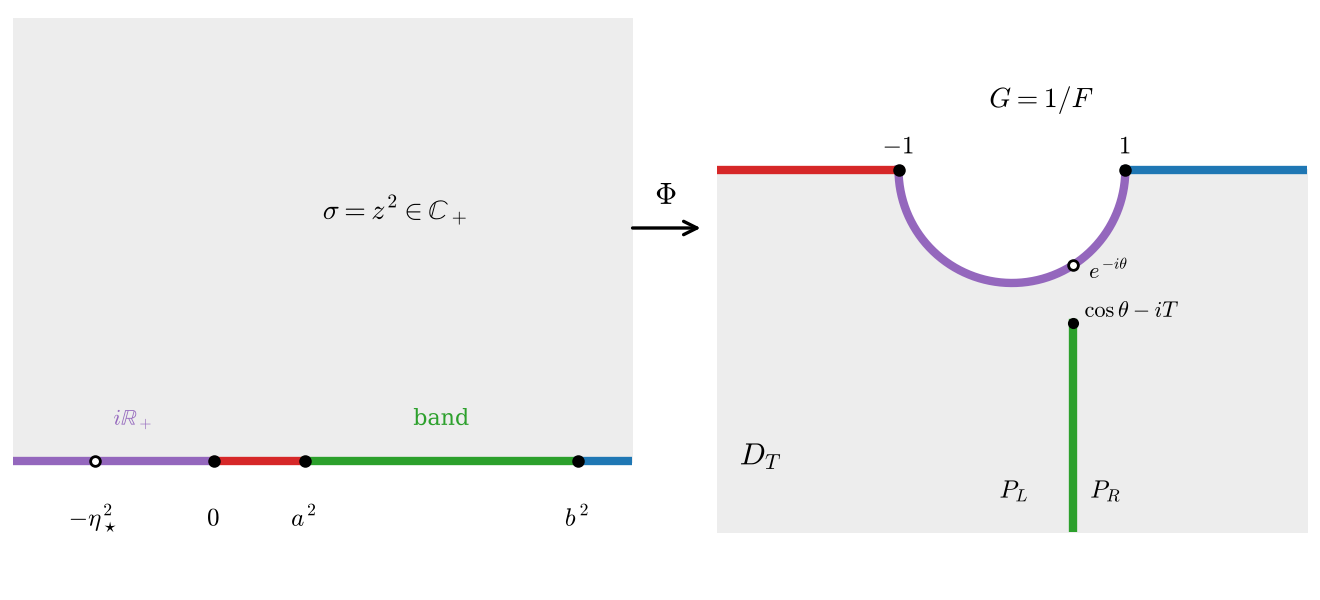
\includegraphics[width=\columnwidth]{figures/fig_slitmap.png}
\caption{The construction of \cref{prop:exist}. Left: the plane of
$\sigma=z^2$, with the boundary arcs coloured. Right: the domain $D_T$ of
$G=1/F$, the part of the lower half-plane outside the unit disc, cut along
the vertical ray $\Re G=\cos\theta$ below the tip $\cos\theta-iT$. The map
$\Phi$ sends each arc on the left to the arc of the same colour; the two ends
of the band go to the two ends of the slit at infinity. The zero of the
optimal system is the preimage of $e^{-i\theta}$.}
\label{fig:slitmap}
\end{figure}

\begin{proposition}\label{prop:exist}
Let $0<\theta<\pi$. There is a system $\Hs$, admissible for $\theta$, with
\eqref{eq:tight}, lossless on $\R\setminus S$, with exactly one zero in
$\Cp$, which is simple and lies on $i\R_+$, and with $\Hs(0)=1$,
$\Hs(iy)\to-1$ as $y\to\infty$, and attenuation positive on $(a,b)$ and zero
at $a$ and $b$.
\end{proposition}

\begin{proof}
For $T>\sin\theta$ let $\Sigma_T=\{\cos\theta-is:\ s\ge T\}$ and
\[
D_T=\{G:\ \Im G<0,\ \abs G>1\}\setminus\Sigma_T .
\]
The ray $\Sigma_T$ does not meet the closed unit disc, since
$\abs{\cos\theta-is}>1$ for $s>\sin\theta$. The domain $D_T$ is simply connected
and its boundary is locally connected, so a conformal map $\Phi$ of $\Cp$
onto $D_T$ extends to a homeomorphism of $\R\cup\{\infty\}$ onto the prime ends
of $D_T$ \cite[Ch.~2]{pommerenke}. Traversed with $D_T$ on the left, the
boundary consists of the lower unit semicircle $C$ from $1$ to $-1$, the ray
$(-\infty,-1]$, the left side of $\Sigma_T$ up to the tip and its right side
down again, and the ray $[1,\infty)$. It has two prime ends at infinity:
$P_L$, between $(-\infty,-1]$ and the left side of the slit, and $P_R$,
between the right side and $[1,\infty)$. We normalise $\Phi$ by $\Phi(\infty)=1$,
$\Phi(0)=-1$ and $\Phi(a^2)=P_L$, and let $s(T)>a^2$ be the preimage of $P_R$.

\emph{Choice of $T$.} Let $\lambda(T)$ be the extremal distance in $D_T$
between $C$ and $\Sigma_T$ \cite[Ch.~4]{ahlforsci}. By conformal invariance it
equals the extremal distance in $\Cp$ between $(-\infty,0)$ and $[a^2,s(T)]$,
which is $L(s(T)/a^2)$ for a continuous strictly decreasing bijection $L$ of
$(1,\infty)$ onto $(0,\infty)$.\footnote{By scaling, $L(\rho)$ is the extremal
distance between $(-\infty,0)$ and $[1,\rho]$. It decreases because the curve
family grows with $\rho$; it tends to $\infty$ as $\rho\to1$, since every curve
crosses the half-annulus $\rho-1<\abs{\sigma-1}<1$, of extremal distance
$\frac1\pi\log\frac1{\rho-1}$; and to $0$ as $\rho\to\infty$, since the half-circles
$\abs\sigma=t$, $1<t<\rho$, join the two sets and have length $\pi t$, which gives
modulus at least $\frac1\pi\log\rho$. Strictness and continuity follow from the
explicit value as a ratio of complete elliptic integrals.} The function
$\lambda$ is continuous in $T$: for $T'$ near $T$ a diffeomorphism
$G\mapsto G-i(T'-T)\chi(G)$, with $\chi$ a smooth bump equal to $1$ near the
tip and supported in a disc around it that avoids the unit circle and the
real axis, maps $D_T$ onto $D_{T'}$ arc by arc, with dilatation
$1+O(\abs{T'-T})$, and extremal distances change at most by that
factor.\footnote{It moves the slit along itself and fixes the rest of the
boundary; it is injective once $\abs{T'-T}\,\abs{\nabla\chi}<1$. A
diffeomorphism whose differential has ratio of singular values at most $K$
changes an extremal distance by a factor in $[1/K,K]$, by transporting the
admissible metrics \cite[Ch.~4]{ahlforsci}.} As $T\to\infty$, every curve in
$D_T$ from $C$ to $\Sigma_T$ crosses the annulus $1<\abs G<T$, so
$\lambda(T)\ge\frac1{2\pi}\log T\to\infty$. As $T\downarrow\sin\theta$, the tip
$\cos\theta-iT$ lies at the distance $\delta=T-\sin\theta$ below the point $e^{-i\theta}$
of $C$, and for $\delta<\rho<\rho_0$ an arc of the circle $\abs{G-e^{-i\theta}}=\rho$
of length less than $2\pi\rho$ joins $C$ to $\Sigma_T$ inside $D_T$; this gives
$\lambda(T)\le2\pi/\log(\rho_0/\delta)\to0$. Hence $s(T)/a^2$ is continuous and
takes every value in $(1,\infty)$, and we fix $T$ with $s(T)=b^2$.

\emph{The system.} On the open first quadrant put $F(z)=1/\Phi(z^2)$, and on
the open second quadrant $F(z)=1/\overline{F(-\bar z)}$. On $i\R_+$, $z^2<0$ is
mapped to $C$, where $\abs\Phi=1$, so the two definitions have the same
continuous boundary values there, and $F$ is analytic in $\Cp$ by Morera's
theorem. $F$ maps $\Cp$ into $\Cp$, since $\Im\Phi<0$, and
$F(-\bar z)=1/\overline{F(z)}$. Define $\Hs$ from $F$ by \eqref{eq:F}. By
\cref{lem:transform}(ii) it is a passive system. On $(0,a)$, $\Phi(t^2)<-1$,
so $F\in(-1,0)$ and $g_\sharp=\pi$; on $(b,\infty)$, $F\in(0,1)$ and $g_\sharp=0$;
in both cases $\abs\Hs=1$. On $(a,b)$, $\Phi(t^2)=\cos\theta-is$ with $s\ge T>\sin\theta$,
which by \eqref{eq:bandcurve} is $H=e^{i\theta-\alpha}$ with
$\coth(\alpha/2)=s/\sin\theta$, so $\alpha>0$, and $\alpha\to0$ at the band edges, where
$s\to\infty$, $F\to0$ and $\Hs\to e^{i\theta}$. Hence $\Hs$ is continuous and
nonzero on a neighbourhood of $[a,b]$, that is, regular on the band, with
argument $\theta$ there. By \cref{lem:transform}(iii) its zeros are the
points with $1/F=e^{-i\theta}$, a point of $C$; $\Phi$ takes this boundary value
at exactly one point of $(-\infty,0)$, and analytically, since $C$ is an
analytic arc, with nonzero derivative. So $\Hs$ has exactly one zero in
$\Cp$, a simple one on $i\R_+$. Finally $\Phi(0)=-1$ gives $F(0)=-1$ and
$\Hs(0)=1$, and $\Phi(\sigma)\to1$ as $\sigma\to-\infty$ gives $\Hs(iy)\to-1$.
\end{proof}

\begin{lemma}\label{lem:identify}
Let $\Hs$ be admissible for $\theta$, with \eqref{eq:tight}, lossless on
$\R\setminus S$, with exactly one zero in $\Cp$, a simple one at $i\eta$, and
with $\Hs(0)=1$ and $\Hs(iy)\to-1$ as $y\to\infty$; for instance the system of
\cref{prop:exist}. Then
$\Hs=-B_\eta e^{ih_g}$ with $g(\omega)=\theta-2\arctan(\omega/\eta)$, $\beta_g=0$, and
the attenuation of $\Hs$ on the band is $v_g$. Consequently $\eta$ is the
root $\eta_\star$ of \eqref{eq:etastar}.
\end{lemma}

\begin{proof}
The quotient $E=\Hs/(-B_\eta)$ is analytic and zero-free in $\Cp$, unimodular
where $\Hs$ is, and bounded, hence bounded by $1$ by the maximum principle, since
$\abs{B_\eta}\to1$ at $\R\cup\{\infty\}$. It has the real symmetry and
$E(0)=\Hs(0)/(-B_\eta(0))=1$, so by \cref{lem:log} $E=e^{ih}$ with an odd
Herglotz function $h$, $h(0)=0$. On $\R\setminus S$, $\abs E=1$, so $\Im h=0$ there:
the measure of $h$ is carried by $S$, and by \eqref{eq:herglotz}, $h$ being
odd, $h(z)=\beta z+O(z^{-1})$ at infinity. Along $[0,a]$ the function $F$ of
$\Hs$ is negative, by \eqref{eq:tight}, with $F(0)=-1$ and $F(a)=0$, so the
argument of $\Hs$ moves continuously from $0$ to $\theta$ inside
$(-\theta,\theta]$,\footnote{The inverse M\"obius map of \eqref{eq:F} sends
$(-\infty,0]$ to the arc of the unit circle from $e^{-i\theta}$ to $e^{i\theta}$
through $1$, with $-1\mapsto1$ and $0\mapsto e^{i\theta}$.} and that of $-B_\eta$ from $0$ to $2\arctan(a/\eta)$ by
\eqref{eq:Bphase}. So on the band $\Re h=\theta-2\arctan(\omega/\eta)=g$, with
no multiple of $2\pi$. The argument of \cref{prop:profile}(iv) now applies
to $h-h_g$: it is real on $\R\setminus S$, has real part $0$ on the band from
above, is continuous up to $S$ (since $E$ is continuous and nonzero near the
band), so $(h-h_g)/R$ is entire, and it is
$O(z^{-1})$ at infinity. Hence $h=h_g$ and $\beta=\beta_g$. Finally
$E(iy)\to(-1)/(-1)=1$, so $h(iy)\to0$ and $\beta=0$. The attenuation is
$\Im h_g=v_g$ on the band. The left side of \eqref{eq:etastar} decreases
strictly in $\eta$ from $\pi\int\dd t/r$ to $0$, so it has exactly one root,
and $\beta_g=0$ says that $\eta$ is this root.
\end{proof}

\begin{proof}[Proof of \cref{thm:allzeros}]
The system $\Hs_\theta=-B_{\eta_\star}e^{ih_{g_\sharp}}$ is the system of
\cref{prop:exist}, by \cref{lem:identify}. This gives (i), with $\as_\theta=v_{g_\sharp}>0$ on the
open band. Since $g_\sharp\ge0$ and decreasing for $\eta\ge\eta_\theta$,
$\beta_{g_\eta}>0$ there (\cref{lem:positivity}); and $\beta_{g_\eta}$ increases
with $\eta$; so $\eta_\star<\eta_\theta$. Part (ii) is \cref{prop:compare}. For
(iii), by \cref{prop:profile}(iii) with $v_{g_\sharp}\ge0$ and $\beta_{g_\sharp}=0$,
$\int_a^b\as_\theta=\frac12\int_a^bg_\sharp\,p$, and the computation in the proof of
\cref{prop:onezero} gives $\theta\Lambda-\delta(\eta_\star)$. It is positive since
$\as_\theta>0$. The systems $H_\eta$ of \cref{prop:onezero} are admissible and
differ from $\Hs_\theta$, since $\beta_{g_\eta}>0$, so by (ii) their mean is
strictly larger. The case $\pi<\theta<2\pi$ follows by passing to $-H$.
\end{proof}

\subsection{Consequences}

\begin{corollary}\label{cor:allweights}
Let $0<\theta<\pi$ and let $H$ be admissible for $\theta$.
\begin{enumerate}
\item[(i)] For every measurable $w\ge0$ on $[a,b]$,
$\int w\alpha\ge\int w\as_\theta$; in particular
$\max_{[a,b]}\alpha\ge\max_{[a,b]}\as_\theta$. The system $\Hs_\theta$ attains all of
these bounds at once.
\item[(ii)] A phase lead costs at least as much as no delay: if $H$ is
passive, regular on the band, and $\arg H\equiv\theta-\tau\omega\pmod{2\pi}$ on
$[a,b]$ for some $\tau\ge0$, then $\alpha\ge\as_\theta$ on $[a,b]$.
\item[(iii)] Every zero-free system with phase $\theta$ on the band, in the
sense of \cref{thm:main}, satisfies $\alpha\ge\as_\theta$ pointwise, in addition
to $\frac1{b-a}\int\alpha\ge\theta\Lambda$.
\end{enumerate}
\end{corollary}

\begin{proof}
(i) is \eqref{eq:pointwise}. (ii) The system $e^{i\tau z}H$ is passive, has
the same modulus on $\R$, and has argument $\theta$ on the band. (iii) is a
special case of (ii) with $\tau=0$.
\end{proof}

Part (i) answers, for systems with zeros allowed, the worst-frequency
question of the zero-free case. Part
(ii) does not extend to a delay, $\arg H=\theta+\tau\omega$ with $\tau>0$: the
system $e^{i\tau z}\Hs_\theta$ still has the loss $\as_\theta$, but it is not
optimal: for $\theta=\pi/2$, $\tau=5$ on $[1,2]$ the least mean loss of a
zero-free system is about forty times smaller (\cref{thm:delay,thm:exactmean}),
and with zeros the least loss falls exponentially in $\tau$ (\cref{cor:rate}).

\begin{corollary}\label{cor:narrowzeros}
Fix $0<\theta<\pi$, and let $f=(a+b)/2$, $\Delta f=b-a$. As $\Delta f/f\to0$,
\[
\Lambda_{\mathrm{all}}(\theta)=\frac\pi8\,\sin\theta\,\frac{\Delta f}f
+O\Big(\Big(\frac{\Delta f}f\Big)^2\Big),
\]
so that $\Lambda_{\mathrm{all}}(\theta)/\theta\Lambda\to\sin\theta/\theta$.
\end{corollary}

\begin{proof}
Write $\epsilon=\Delta f/f$. By \eqref{eq:intro-bounds}, $\Lambda=\frac\pi8\epsilon+O(\epsilon^3)$.
By the proof of \cref{prop:onezero}, $\int_a^bp=J=2(b-a)\Lambda$, and by
\cref{lem:moments}(i), $\int_a^b\omega p=0$, so
$\frac1{b-a}\int_a^b(\omega-f)p=-2f\Lambda$. Taylor's formula for
$\arctan(\omega/\eta)$ at $\omega=f$, with a remainder $O((\omega-f)^2/\eta^2)$ that
is integrated against $\abs p$, whose mean over the band is
$O(1)$,\footnote{In $\omega=f+\frac{\Delta f}2s$, $p\,\dd\omega/(b-a)=-s\,\dd s/\sqrt{1-s^2}\,(1+O(\epsilon))$.}
gives
\[
\delta(\eta)=2\Lambda\arctan\frac f\eta-2\Lambda\frac{f\eta}{f^2+\eta^2}
+O\Big(\frac{\epsilon^2f^2}{\eta^2}\Big).
\]
The root of \eqref{eq:etastar} satisfies $2\arctan(f/\eta_\star)=\theta+O(\epsilon)$,
since the weight $\dd t/r$ is carried by an interval of length $\epsilon f$
around $f$. With $\phi=2\arctan(f/\eta_\star)$ and
$2f\eta/(f^2+\eta^2)=\sin\phi$,
\begin{align*}
\Lambda_{\mathrm{all}}&=\theta\Lambda-\delta(\eta_\star)=\Lambda\,(\theta-\phi+\sin\phi)+O(\epsilon^2)\\
&=\Lambda\sin\theta+O(\epsilon^2),
\end{align*}
because $\Lambda=O(\epsilon)$ and $\theta-\phi=O(\epsilon)$; also $f/\eta_\star$ stays
bounded.
\end{proof}

In the computations (\cref{app:verification}) the relative error is of the
order of $(\Delta f/f)^2$: the ratio of $\Lambda_{\mathrm{all}}$ to the leading
term is $1.0021$ for $b/a=1.2$ and $1.000149$ for $b/a=1.05$ at $\theta=\pi/2$.
For small phases zeros hardly help: the gain is a factor
$\sin\theta/\theta=1-\theta^2/6+\dots$. For the $1^\circ$ shift at $5$\,MHz of
\cref{sec:waves}, the least mean attenuation with zeros allowed is
$1.37588\times10^{-3}$\,Np, against $1.37595\times10^{-3}$\,Np without zeros.

For general $\theta$ the profile $\as_\theta$ is elliptic, not elementary
(\cref{ssec:closedform}), and a simple bound with the right shape survives, for the equilibrium weight of the band
\[
w_0(\omega)=\frac1{I_0\,r(\omega)},\qquad I_0=\int_a^b\frac{\dd t}{r(t)}=\frac{K(k)}b ,
\]
$k^2=1-a^2/b^2$.

\begin{corollary}\label{cor:nome}
Let $0<\theta<\pi$ and let $H$ be admissible for $\theta$. Then
\begin{equation}\label{eq:nome}
\int_a^bw_0\log\tanh\frac\alpha2\dd\omega\ \ge\ \log\sin\theta-\pi\frac{K(a/b)}{K(k)} ,
\end{equation}
that is, the $w_0$-geometric mean of $\tanh(\alpha/2)$ is at least
$q\sin\theta$, where $q=e^{-\pi K(a/b)/K(k)}$ is the nome of the modulus $k$.
Equality holds if and only if $\theta=\pi/2$ and $H=\Hs_{\pi/2}$. For an octave
$q=0.085796$, for a decade $q=0.26220$.
\end{corollary}

\begin{proof}
By \cref{lem:transform}(iv), $\tanh(\alpha/2)=e^u\sin\theta/\sin v\ge e^u\sin\theta$,
with equality only where $v=\pi/2$, which requires $\theta=\pi/2$. Let
$\zeta_0$ be the function in the proof of \cref{thm:rightangle} and
$d=\zeta-\zeta_0$, so that $\Im d=g-g_0$, which is $\le0$ on $(0,a)$ and $\ge0$
on $(b,\infty)$. Both functions have the form \eqref{eq:zetarep}, so
$\Re d(x)=\frac1\pi\PV\int_0^\infty\Im d(t)\,\frac{2x}{t^2-x^2}\dd t$ almost
everywhere. Integrating against $w_0$ and exchanging the integrals, by
Tonelli's theorem for $t\notin(a,b)$ and by the antisymmetry of the Hilbert
transform between $L^p$ and $L^{p'}$ for $t\in(a,b)$ ($\Im d$ is bounded and
$w_0\in L^{p'}$ for $p'<2$), gives
\begin{gather*}
\int_a^bw_0\Re d=\frac1\pi\int_0^\infty\Im d(t)\,k_0(t)\dd t,\\
k_0(t)=\PV\int_a^b\frac{2x\,w_0(x)}{t^2-x^2}\dd x .
\end{gather*}
In $\sigma=x^2$,
\[
k_0(t)=\frac1{I_0}\,\PV\int_{a^2}^{b^2}\frac{\dd\sigma}{(t^2-\sigma)\sqrt{(\sigma-a^2)(b^2-\sigma)}},
\]
which vanishes for $a<t<b$ by Glauert's integral (proof of
\cref{lem:positivity}), is negative for $t<a$ and positive for $t>b$. So
$\int w_0\Re d\ge0$, with equality only if $g=g_0$ off the band. For
$\zeta_0$ the same computation, with $g_0$ explicit, gives
\begin{align*}
\int_a^bw_0\Re\zeta_0&=\int_0^ak_0(t)\dd t\\
&=-\frac\pi{I_0}\int_0^a\frac{\dd t}{\sqrt{(a^2-t^2)(b^2-t^2)}} ,
\end{align*}
using, for $s<A$,
\[
\int_A^B\frac{\dd\sigma}{(\sigma-s)\sqrt{(\sigma-A)(B-\sigma)}}=\frac\pi{\sqrt{(A-s)(B-s)}} ;
\]
the last integral is $K(a/b)/b$.\footnote{Substitute $t=a\sin\phi$: then $\sqrt{(a^2-t^2)(b^2-t^2)}$ is
$a\cos\phi\cdot b\sqrt{1-(a/b)^2\sin^2\phi}$ and $\dd t=a\cos\phi\dd\phi$.
Similarly $I_0=K(k)/b$ by $t^2=b^2-(b^2-a^2)\sin^2\phi$.} Adding up gives \eqref{eq:nome}.
\end{proof}

\subsection{The optimum in closed form}\label{ssec:closedform}

The profile $\as_\theta$ is elliptic for every $\theta$.\footnote{The route
goes through \cref{lem:zeroatom}: the zero of $\Hs_\theta$ becomes an
integral over $u$ of explicit algebraic functions, and the integral over $u$
in \eqref{eq:hsharpexplicit} is an elliptic integral of the third kind.} Write $\operatorname{sn}$,
$\operatorname{cn}$ and $\operatorname{am}$ for the Jacobi functions of
modulus $k$, $k^2=1-a^2/b^2$ \cite[Ch.~22]{dlmf}, $F(\psi,k)$ for the
incomplete integral of the first kind, and
\[
\Pi(n;\psi,k)=\int_0^\psi\frac{\dd v}{(1-n\sin^2v)\sqrt{1-k^2\sin^2v}},
\]
with $\Pi(n,k)=\Pi(n;\pi/2,k)$. For $u\ge0$ put
$Q_u=\sqrt{(u^2+a^2)(u^2+b^2)}$, so that $R(iu)=-Q_u$ by \cref{lem:R} and
continuity from $R(0)=-ab$.

\begin{lemma}\label{lem:zeroatom}
For $u>0$ let $j_u(t)=t/(t^2+u^2)$. Then
\[
h_{j_u}(z)=\frac z{z^2+u^2}\Big(1+\frac{R(z)}{Q_u}\Big),\qquad
\beta_{j_u}=\frac1{Q_u},
\]
and $v_{j_u}(x)=x\,r(x)/((x^2+u^2)Q_u)$ on the band.
\end{lemma}

\begin{proof}
Call the right side $\phi_u$. It is odd, real on $\R\setminus S$, analytic
off $S$, since its apparent poles at $\pm iu$ cancel ($1+R(\pm iu)/Q_u=0$),
continuous up to $S$, and $\phi_u(z)=z/Q_u+O(z^{-1})$. On the band
$\Re\phi_u(x+i0)=j_u(x)$, because $R(x+i0)=ir(x)$. By the substitution
$\sigma=t^2$ and the integral displayed in the proof of \cref{cor:nome},
$\beta_{j_u}=\frac1\pi\int_{a^2}^{b^2}\dd\sigma/((\sigma+u^2)
\sqrt{(\sigma-a^2)(b^2-\sigma)})=1/Q_u$. So $\phi_u-h_{j_u}$ has real part
$0$ on the band and is $O(z^{-1})$ at infinity, and the argument of the proof
of \cref{prop:profile}(iv) gives $\phi_u=h_{j_u}$.
\end{proof}

Since $\arctan(t/\eta)=\frac\pi2-\int_0^\eta j_u(t)\dd u$, the phase of
\cref{thm:allzeros} is $g_\sharp=\theta-\pi+2\int_0^{\eta_\star}j_u\dd u$, and
by linearity
\begin{equation}\label{eq:hsharpexplicit}
h_{g_\sharp}=(\theta-\pi)h_\circ+2\arctan\frac{\eta_\star}z
+2zR(z)\int_0^{\eta_\star}\frac{\dd u}{(z^2+u^2)Q_u},
\end{equation}
with $h_\circ$ and $A$ as in \cref{sec:pointwise}. In particular
\begin{equation}\label{eq:asharpP}
\as_\theta(x)=2x\,r(x)\int_0^{\eta_\star}\frac{\dd u}{(x^2+u^2)Q_u}-(\pi-\theta)A(x).
\end{equation}
A zero of $H$ at $iu$ thus acts on the band as a measure at the negative
squared frequency $-u^2$; this is the mechanism behind \cref{sec:beyond}.

\begin{theorem}\label{thm:etaexplicit}
Let $0<\theta<\pi$. The root of \eqref{eq:etastar} is
\begin{equation}\label{eq:etaexplicit}
\eta_\star=b\,\frac{\operatorname{cn}(u_\theta,k)}{\operatorname{sn}(u_\theta,k)},\qquad
u_\theta=\frac{\theta K(k)}\pi .
\end{equation}
\end{theorem}

\begin{proof}
By \eqref{eq:hsharpexplicit}, $\beta_{g_\sharp}=(\theta-\pi)\tau_\circ
+2\int_0^{\eta_\star}\dd u/Q_u$, and \eqref{eq:etastar} says
$\beta_{g_\sharp}=0$. The substitution $u=b\cot\phi$ gives
$\dd u/Q_u=-\dd\phi/(b\sqrt{1-k^2\sin^2\phi})$, since
$u^2+a^2=b^2(1-k^2\sin^2\phi)/\sin^2\phi$, so
\[
\int_\eta^\infty\frac{\dd u}{Q_u}=\frac1bF\Big(\arctan\frac b\eta,k\Big),
\qquad \int_0^\infty\frac{\dd u}{Q_u}=\frac{K(k)}b .
\]
With $\tau_\circ=2K(k)/(\pi b)$ the equation becomes
\[
F\big(\arctan(b/\eta_\star),k\big)=\theta K(k)/\pi,
\]
that is, $\arctan(b/\eta_\star)=\operatorname{am}(u_\theta,k)$.
\end{proof}

At $\theta=\pi/2$, $\operatorname{cn}/\operatorname{sn}$ at $K/2$ is
$\sqrt{k'}=\sqrt{a/b}$, and $\eta_\star=\sqrt{ab}$ as in \cref{thm:rightangle}.
Put $\eta=\eta_\star$ and
\begin{equation}\label{eq:ellipticparam}
Q=Q_\eta,\qquad n=\frac{b^2-a^2}{b^2+\eta^2},\qquad
c_\theta=\frac{\Pi(n,k)}{(b^2+\eta^2)K(k)} .
\end{equation}

\begin{theorem}\label{thm:ellipticprofile}
Let $0<\theta<\pi$. On the band,
\begin{gather}
\as_\theta(x)=\frac{2\eta Q}b\Big(c_\theta F(\psi,k)-\frac{\Pi(n;\psi,k)}{b^2+\eta^2}\Big),
\label{eq:alphaelliptic}\\
\sin^2\psi=\frac{b^2-x^2}{b^2-a^2},\qquad 0\le\psi\le\frac\pi2,\notag\\
\frac{\dd\as_\theta}{\dd x}=\frac{2\eta Q}{r(x)}\Big(\frac1{x^2+\eta^2}-c_\theta\Big).
\label{eq:alphaellipticprime}
\end{gather}
The profile has a single maximum, at $x_\theta=\sqrt{1/c_\theta-\eta^2}$, and
\begin{equation}\label{eq:ellipticmean}
\Lambda_{\mathrm{all}}(\theta)=\frac{\pi\eta}{b-a}\,(Qc_\theta-1).
\end{equation}
Near $z=0$, with $z=a\sin\phi$ and $\phi(0)=0$,
\begin{equation}\label{eq:transferelliptic}
\Hs_\theta(z)=\exp\Big[\frac{2iQ}{b\eta}\Big(\Pi\Big(-\frac{a^2}{\eta^2};\phi,\frac ab\Big)
-\eta^2c_\theta F\Big(\phi,\frac ab\Big)\Big)\Big].
\end{equation}
\end{theorem}

\begin{proof}
Let $h=h_{g_\sharp}$ and $\Psi(z)=R(z)\big(h'(z)+2\eta/(z^2+\eta^2)\big)$. The
function $g_\sharp$ extends analytically to the strip $\abs{\Im z}<\eta$, and
$h-g_\sharp$ has real part $0$ on the band, so by Schwarz reflection $h$
continues analytically across $(a,b)$ and $h'(x+i0)=g_\sharp'(x)+i\as'(x)$
with $g_\sharp'=-2\eta/(x^2+\eta^2)$. Hence $\Psi(x+i0)=-r(x)\as'(x)$ is real,
and by the symmetry $h(\bar z)=\overline{h(z)}$ it equals $\Psi(x-i0)$; so
$\Psi$ has no jump across the band, nor, being even, across $(-b,-a)$. Near
the ends of $S$, \eqref{eq:hsharpexplicit} gives
\[
\Psi=(\theta-\pi)\tau_\circ(z^2-m^2)+2R^2I+2zRR'I+2zR^2I',
\]
with $I(z)=\int_0^\eta\dd u/((z^2+u^2)Q_u)$, which is analytic near
$\pm a,\pm b$, and $RR'=z(2z^2-a^2-b^2)$; so $\Psi$ is bounded there and the
ends are removable. Since $h$ is analytic off $S$, the only other
singularities of $\Psi$ are at $\pm i\eta$, from the term $2\eta R/(z^2+\eta^2)$,
and since $R(\pm i\eta)=-Q$, the function $\Psi+2\eta Q/(z^2+\eta^2)$ is
entire. At infinity $h=O(z^{-1})$, because $\beta_{g_\sharp}=0$, so
$h'=O(z^{-2})$ and $\Psi$ is bounded. Hence $\Psi=d-2\eta Q/(z^2+\eta^2)$ for a constant $d$, and
\[
h'(z)=-\frac{2\eta}{z^2+\eta^2}+\frac{d-2\eta Q/(z^2+\eta^2)}{R(z)} .
\]
On the band, $\as'=-\Psi/r$ gives \eqref{eq:alphaellipticprime} with $d=2\eta
Qc$ for some $c$. Since $\as$ vanishes at $a$ and $b$ (\cref{thm:allzeros}),
$\int_a^b\as'=0$ and $c=\int_a^b\dd t/((t^2+\eta^2)r)\big/\int_a^b\dd t/r$.
The substitution $t=b\sqrt{1-k^2\sin^2v}$, for which $\dd t/r=-\dd v/t$ and
$t^2+\eta^2=(b^2+\eta^2)(1-n\sin^2v)$, gives $c=c_\theta$, and integrating
\eqref{eq:alphaellipticprime} from $x$ to $b$ gives \eqref{eq:alphaelliptic}.
As $c_\theta$ is a strict average of $(t^2+\eta^2)^{-1}$ over the band,
$\as'$ changes sign once, at $x_\theta$. At infinity
$h'=2\eta(Qc_\theta-1)z^{-2}+O(z^{-4})$, so $h=-2\eta(Qc_\theta-1)/z+O(z^{-3})$,
while by \eqref{eq:foster} with no measure off $S$,
$h=-\frac2\pi\int_a^b\as/z+O(z^{-3})$; this gives \eqref{eq:ellipticmean}.
Finally $\Hs_\theta=-B_\eta e^{ih}$, $B_\eta'/B_\eta=2i\eta/(z^2+\eta^2)$, so
\[
\frac{(\Hs_\theta)'}{\Hs_\theta}=\frac{2i\eta Q}{R(z)}\Big(c_\theta-\frac1{z^2+\eta^2}\Big),
\]
and $\Hs_\theta(0)=1$. Near $0$ put $z=a\sin\phi$; then
$R=-ab\cos\phi\sqrt{1-(a/b)^2\sin^2\phi}$ and
$z^2+\eta^2=\eta^2(1+(a/\eta)^2\sin^2\phi)$, and integrating gives
\eqref{eq:transferelliptic}.
\end{proof}

The formula \eqref{eq:transferelliptic} holds near the origin and is
continued analytically along paths in $\C\setminus S$; the residue $1$ of
the logarithmic derivative at $i\eta$ makes the continuation single-valued
with a simple zero there. At $\theta=\pi/2$, \cref{thm:ellipticprofile}
reduces to \cref{thm:rightangle}: $c_{\pi/2}=1/(2ab)$, $x_\theta=\sqrt{ab}$
and $\Lambda_{\mathrm{all}}(\pi/2)=\frac\pi2(\sqrt b-\sqrt a)/(\sqrt b+\sqrt a)$.
The values of \cref{tab:allzeros} follow from \eqref{eq:etaexplicit},
\eqref{eq:ellipticmean} and $x_\theta$ without any root finding.
